\subsection{Building Generation}
The purpose of the BuildingGenerator is to generate different kinds of visually pleasing buildings, everything from small houses to towering Manhattan-style skyscrapers. 
The BuildingGenerator has three inputs: the plot in which to build, the terrain on which to build on top of, and the population scalar that helps determine the size of the building.
The function spawns a building into the world. 

\begin{table}[H]
    \centering
    \begin{tabular}{lllll}
      \textbf{Input}                           &               & \textbf{Function}            &               & \textbf{Output}         \\
      \midrule
      \textit{Plot, Terrain, Population}       & $\rightarrow$ & \textbf{BuildingGenerator}   & $\rightarrow$ & \textit{Building}       \\
      \bottomrule
    \end{tabular}
 
    \caption{Definition of the BlockGenerator function, which is responsible for constructing a single building on top of a plot.}
    \label{table:buildinggen}
  \end{table}
  \vspace{-0.4cm} 

Seeing as buildings are one of the most important parts of generating a convincing modern city, it is essential to have a generator that can create different kinds of buildings. 
The problem of creating many different kinds of buildings was broken down into several different sub-generators, each responsible for a particular type of building.
The plot label helps decide what kind of sub-generator to use. 
The different sub-generators then have to take the inputs into account to generate a building.

% There are two different strategies implemented in this project for generating buildings: Using an L-system or importing an existing model of a building. 

% manhattan typ aktiga byggnader passar bra här
Multiple L-systems with a stochastic grammar were used to generate a unique set of buildings. 
The L-systems were implemented with type parameters to be able to handle the generation of any object, such as walls or floors.
The two types of parameters are the object type in the L-system and the data class that is used for the generation.
A building generated via L-systems has some generated floors, where each floor has walls and is built with multiple smaller textured wall segments. 
Examples of wall segments can be shop windows, normal windows, and doors.
The steps for generating a Manhattan-style skyscraper are as follows:
\begin{enumerate}
    \item An L-system is used to generate different kinds of floors for the building. Note that these floor types indicate what kind of L-system should be used later for the generation of the wall segments. Example of floor types can be:
    \begin{itemize}
        \item FirstFloor - A floor that has Shop Windows and Doors
        \item OnlyWindowFloor - A floor that will only have window segments. 
        \item MirrorFloor - Generate half of the floor segments and then copy and flip it for the next half of floor segments.
    \end{itemize}
    Images of these floor labels can be found in Figure \ref{fig:segmentsgen}.
    \item Each wall is then generated, floor-by-floor. Each floor type has its own L-system to generate different wall segments.
    \item After every wall has been generated; the building is put together inside the plot.
    \item A flat roof is generated at the top of the building.
    \item The building is then placed on the highest point of the terrain within the plot. Basement walls are then generated downwards to not make the building float in the air. %techically it's the highest point of the plot.points
\end{enumerate}

% Explain how the direction of the wall is decide. Maybe draw a picture of it?

% Add FirstFloor, OnlyWindowFloor and MirrorFloor images

\begin{figure}[H]
  \centering
  \begin{subfigure}[b]{0.32\textwidth}
    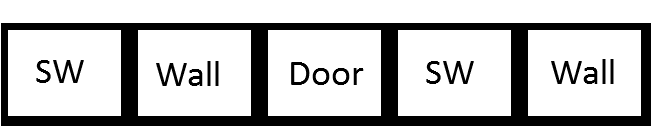
\includegraphics[width=\textwidth]{figure/FirstFloor.png}
    \caption{FirstFloor.}
  \end{subfigure}
  \quad
  \begin{subfigure}[b]{0.32\textwidth}
    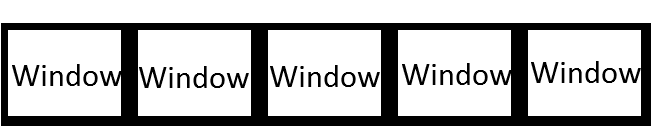
\includegraphics[width=\textwidth]{figure/OnlyWindowFloor.png}
    \caption{OnlyWindowFloor.}
  \end{subfigure}
  \begin{subfigure}[b]{0.32\textwidth}
    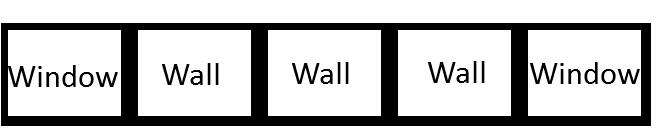
\includegraphics[width=\textwidth]{figure/MirrorFloor.png}
    \caption{MirrorFloor.}
  \end{subfigure}

  \caption{Three different floor types and an example of their wall segment generation}
  \label{fig:segmentsgen}
\end{figure}
